% !TEX root = ../vr_st.tex

\subsection{First critical values}\label{sub:general_barcodes}

%Let $X$ be an $\R$-space where $X_r$ is empty for $r<0$ and contractible for $r\geq R$ for some real number $R$.
%The Vietoris--Rips complex of a metric space is our primary example.
%In this subsection, we will consider this $\R$-space and omit it from the notation when convenient.

\subsubsection{}\label{subsub:first_critical_value}\label{subsub:beta v.s. fillrad}

Let $X$ be an $\R$-space where $X_r$ is empty for $r<0$ and contractible for $r \geq R$ for some real number $R$.
The Vietoris--Rips complex of a metric space is our primary example.
The \defn{first critical value} of the $\R$-space $X$ is the supremum among real numbers $r$ such that $X_{s,t}$ is a homotopy equivalence for any $s,t \in [0,r]$. \ling{change throughtout the paper that the filtration is open Vietoris-Rips.}

\ling{use reduced homology.}

The \defn{first critical value} of a persistence module which is \(0\) for negative numbers, is defined as the smallest value \(\beta\) such that \((0, \beta)\) appears as a bar in the barcode of the persistence module.\anibal{Careful with the open vs closed interval here}

Clearly, the first critical value of an $\R$-space is bounded above by the first critical value of its $\degp^\th$ homology, as well as that of \(\img\theta\) and \(\ker\theta\) for any linear cohomology operation $\theta$.
In addition, all these critical values are bounded above by $R$.

\subsubsection{}\label{l:crit_val and fill_rad 1}

\lemma Let $\cX$ be a closed $n$-manifold which is orientable with \(\k\)-coefficients.
If \(\beta_n\) denotes the first critical value of \(\rH_n(\VR(\cX); \k)\) then
\[
\beta_m \leq 2 \cdot \fillrad(\cX; \k).
\]

\begin{proof}
	This follows directly from the lemma in \cref{ss:filling_radius}.
\end{proof}

%\medskip Recall from \cref{ss:filling_radius} that $\VR_{2\bullet}(\cX)$ and the Kuratowski filtration $U_\bullet(\cX)$ are (filtered) homotopy equivalent.
%By the definition of the filling radius, it follows that the first critical value of the $n^\th$ homology of $\VR(\cX)$ is at most $2\fillradnofield{\cX}$.

\subsubsection{}\label{subsub:barcode_general}

Let $X$ be an $\R$-space as before.
Let \(\degp \in \N\) and \(\theta \in \cO(\ell,\degp)\) a linear cohomology operation.
We respectively denote by $\alpha, \beta_\degp$ and $\gamma_\theta$ the first critical values of $X$, \(\rH_\degp(X)\), and \(\img_\theta(X)\).\anibal{It should be \(\gamma_\theta\) not \(\gamma_\degp\).
	Additionally, We should talk about \(\img_\theta\)-barcodes not \(\theta\)-barcodes since this analysis is not been carried through for \(\ker_\theta\). Or is it?}
 \ling{Follow this convention and unify notation.}

Because the $\R$-space $X$ is empty for \(r < 0\) and the homotopy type of $X_r$ remains unchanged for $r \in [0, \alpha)$, bars in \(\barc \rH_\degp(X)\) and $\barc\img_\theta(X)$ either start at $0$ or start after $\alpha$.

%In addition, for degrees $\degp$ such that $\rH_\degp(X_0)$ is non-trivial, the barcode of the $\degp^\th$ homology of $X$ always contains $(0,\beta_\degp)$.
%More precisely,
Furthermore, if \(k = \dim \opH_\degp(X_0) > 0\) then the $\barc\rH_\degp X$ contains $(0,\beta_m)$ and \((k - 1)\) additional bars of the form \((0, a)\) for \(a \in [\beta_\degp, R]\), along with possibly more bars dominated by \((\alpha, \pi)\).

\ling{continue editting}

if ...

Similarly, if ...

$\theta$-barcodes of $X$, where $\theta\in\cO(\ell,\degp)$ is a linear cohomology operation; the leftmost one contains one \((0, \gamma_m)\) and \((\dim \img \theta_{X_0} - 1)\) additional bars of the form \((0, b)\) for \(b \in [\beta_\degp, R]\), along with possibly more bars dominated by \((\alpha, \pi)\).

and if ...

Please consult \cref{fig:barcodes_general} for a depiction of these four barcode estimates.

\begin{figure}
	\centering
	\begin{tikzpicture}[scale=0.52]
	\begin{axis} [
		title = {\LARGE $\barc\opH_m^{\VR}(\cM)$, if $\opH_m(\cM) \neq 0$},
		ticklabel style = {font=\Large},
		axis y line=middle,
		axis x line=middle,
		ytick={0.7,0.95},
		yticklabels={$2\firstdeath{m}{\cM}$,$\diam(\cM)$},
		xtick={0.55,0.95},
		xticklabels={$2\crit(\cM)$, $\diam(\cM)$},
		xmin=-0.015, xmax=1.1,
		ymin=0, ymax=1.1,]
		\addplot [mark=none] coordinates {(0,0) (1,1)};
		\addplot [thick,color=black!20!white,fill=black!30!white,
		fill opacity=0.4]coordinates {
			(0.55,0.95)
			(0.55,0.55)
			(0.95,0.95)
			(0.55,0.95)};
		\addplot [black!40!white,mark=none,dashed, thin] coordinates {(0,0.7) (0.7,0.7)};
		\addplot [black!40!white,mark=none,dashed, thin] coordinates {(0,0.55) (0.55,0.55)};
		\addplot [black!40!white,mark=none,dashed, thin] coordinates {(0.55,0) (0.55,0.55)};
		\addplot[line width=1.5mm, color=black!30!white] coordinates{(0, 0.7) (0, 0.95)};
		\addplot[barccolor,mark=*] (0, 0.7) circle (2pt) node[above right,barccolor]{};
	\end{axis}
\end{tikzpicture}
\begin{tikzpicture}[scale=0.52]
	\begin{axis} [
		title = {\LARGE $\barc\opH_m^{\VR}(\cM)$, if $\opH_m(\cM) = 0$},
		ticklabel style = {font=\Large},
		axis y line=middle,
		axis x line=middle,
		ytick={0.95},
		yticklabels={$\diam(\cM)$},
		xtick={0.55,0.95},
		xticklabels={$2\crit(\cM)$, $\diam(\cM)$},
		xmin=-0.015, xmax=1.1,
		ymin=0, ymax=1.1,]
		\addplot [mark=none] coordinates {(0,0) (1,1)};
		\addplot [thick,color=black!20!white,fill=black!30!white,
		fill opacity=0.4]coordinates {
			(0.55,0.95)
			(0.55,0.55)
			(0.95,0.95)
			(0.55,0.95)};
		\addplot [black!40!white,mark=none,dashed, thin] coordinates {(0,0.55) (0.55,0.55)};
		\addplot [black!40!white,mark=none,dashed, thin] coordinates {(0.55,0) (0.55,0.55)};
	\end{axis}
\end{tikzpicture}

\begin{tikzpicture}[scale=0.52]
	\begin{axis} [
		title={\LARGE $\thetabarc{\cM}$, if $\img\theta_{\cM}\neq 0$},
		ticklabel style = {font=\Large},
		axis y line=middle,
		axis x line=middle,
		ytick={0.7,0.95},
		yticklabels={$2\firstdeath{\theta}{\cM}$,$\diam(\cM)$},
		xtick={0.55,0.95},
		xticklabels={$2\crit(\cM)$, $\diam(\cM)$},
		xmin=-0.015, xmax=1.1,
		ymin=0, ymax=1.1,]
		\addplot [mark=none] coordinates {(0,0) (1,1)};
		\addplot [thick,color=black!20!white,fill=black!30!white,
		fill opacity=0.4]coordinates {
			(0.55,0.95)
			(0.55,0.55)
			(0.95,0.95)
			(0.55,0.95)};
		\addplot [black!40!white,mark=none,dashed, thin] coordinates {(0,0.7) (0.7,0.7)};
		\addplot [black!40!white,mark=none,dashed, thin] coordinates {(0,0.55) (0.55,0.55)};
		\addplot [black!40!white,mark=none,dashed, thin] coordinates {(0.55,0) (0.55,0.55)};
		\addplot[line width=1.5mm, color=black!30!white] coordinates{(0, 0.7) (0, 0.95)};
		\addplot[barccolor,mark=*] (0, 0.7) circle (2pt) node[above right,barccolor]{};
	\end{axis}
\end{tikzpicture}
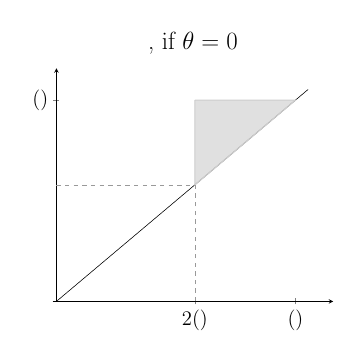
\begin{tikzpicture}[scale=0.52]
	\begin{axis} [
		title={\LARGE $\thetabarc{\cM}$, if $\img\theta_{\cM}= 0$},
		ticklabel style = {font=\Large},
		axis y line=middle,
		axis x line=middle,
		ytick={0.95},
		yticklabels={$\diam(\cM)$},
		xtick={0.55,0.95},
		xticklabels={$2\crit(\cM)$, $\diam(\cM)$},
		xmin=-0.015, xmax=1.1,
		ymin=0, ymax=1.1,]
		\addplot [mark=none] coordinates {(0,0) (1,1)};
		\addplot [thick,color=black!20!white,fill=black!30!white,
		fill opacity=0.4]coordinates {
			(0.55,0.95)
			(0.55,0.55)
			(0.95,0.95)
			(0.55,0.95)};
		\addplot [black!40!white,mark=none,dashed, thin] coordinates {(0,0.55) (0.55,0.55)};
		\addplot [black!40!white,mark=none,dashed, thin] coordinates {(0.55,0) (0.55,0.55)};
	\end{axis}
\end{tikzpicture}
	\caption{In each figure the gray region represents where additional bars could potentially exist within the corresponding barcode.}
	\anibal{Instead of additional points I would use a gray region in the y axis. \ling{Done.}}
	\label{fig:barcodes_general}
\end{figure}